Usability testing refers to evaluating a product or service by testing it with representative users. In principle, during a usability test, participants  will evaluate the system with quantitative metrics. 

The goal of usability testing is to collect the quantitative data, analyze the result and issue the usability problems with tested system. 

\subsection{System Usability Scale}

The System Usability Scale (SUS) offers a "quick and dirty", but relative reliable approach for measuring the usability\cite{brooke1996sus}.  It contains a 10 item questionnaire with five rating options for participants; from \textit{strongly agree} to \textit{strongly disagree}.


In order to calculate the SUS score, score contributions from each item should be calculated once separately at first. The score contribution will range from 0 to 4. For items with odd number, the score contribution should minus 1. For item with an even number, the contribution is 5 minus the score. The sum of all scores is multiplied by 2.5 to obtain the overall value of SUS, which has a range of 0 to 100.

\begin{equation}
\label{formular:SUS}
SUS_{sum} = 2.5 \times \left (  \sum_{ i=1}^{5} \left ( a_{2i-1} - 1 \right ) + \sum_{ i=1}^{5} \left ( 5 - a_{2i} \right ) \right ) 
\end{equation}


\begin{table}[!htbp]
\centering
\begin{tabularx}{\textwidth}{@{}lXXXXXl@{}}
\toprule
Item(No.)   & A  & B  & C  & D  & E          & Average Score        \\ \midrule
1               & 3  & 4  & 3  & 4  & 4          & 3.6                     \\
2               & 2  & 1  & 1  & 1  & 2          & 1.4                     \\
3               & 5  & 4  & 4  & 5  & 4          & 4.4                     \\
4               & 1  & 2  & 1  & 2  & 2          & 1.6                     \\
5               & 4  & 4  & 3  & 4  & 5          & 4                     \\
6               & 4  & 5  & 4  & 3  & 4          & 4                     \\
7               & 5  & 4  & 4  & 5  & 5          & 4.6                     \\
8               & 3  & 3  & 2  & 1  & 3          & 2.4                     \\
9               & 5  & 4  & 3  & 4  & 5          & 4.2                     \\
10              & 2  & 3  & 2  & 1  & 2          & 2                     \\ \bottomrule        
\end{tabularx}
\caption{Score of SUS table}
\label{table:score-sus}
\end{table}

For the SUS testing of Graphicuss system, 5 participants are involved in the interview with SUS questionnaire, which is listed in appendix \ref{appendix:sus}. Each participant gives his own score contribution for each item, and the average score of each item is calculated. Table \ref{table:score-sus} shows the result.

According to the formula \ref{formular:SUS}, the final sum SUS score of the system is \textbf{73.5}. An article represents the mapping of adjective ratings to SUS score\cite{bangor2009determining}. And a \textbf{73.5} SUS score achieves the rating in a range of \textit{Good} to \textit{Excellent} when it is expressed by adjective ratings. 

The result reveals that the Graphicuss system achieves a relative high score in the general usability test. In general, users are able to learn to use this system very quickly. Without significant help, they can operate the system smoothly and unproblematically. 

% \cite{bangor2009determining} \cite{gackenheimer2015core}\cite{barron1998minimum}\cite{grunwald2005advances}\cite{ferraiolo2000scalable}\cite{fette2011websocket}\cite{geary2012core}\cite{richardson2008restful}\cite{pautasso2008restful}\cite{pimentel2012communicating}



\subsection{Interview based Usability Test}

Interviews with college students have been conducted in order to evaluate the system's usability as well as the fulfillment of requirements. 

Nielsen had a research about the relationship between the amount of test users and the percentage of problems they found. Figure \ref{fig:eval-nielsen} shows the result\cite{nielsen2001conduct}. Only 5 participants are already enough for discovering 75\% of usability problems in most cases. Therefore, for the interview of evaluation, 5 participants are invited. The key parameters of the interview are listed as follows. 

\begin{figure}[!htbp]
  \centering
    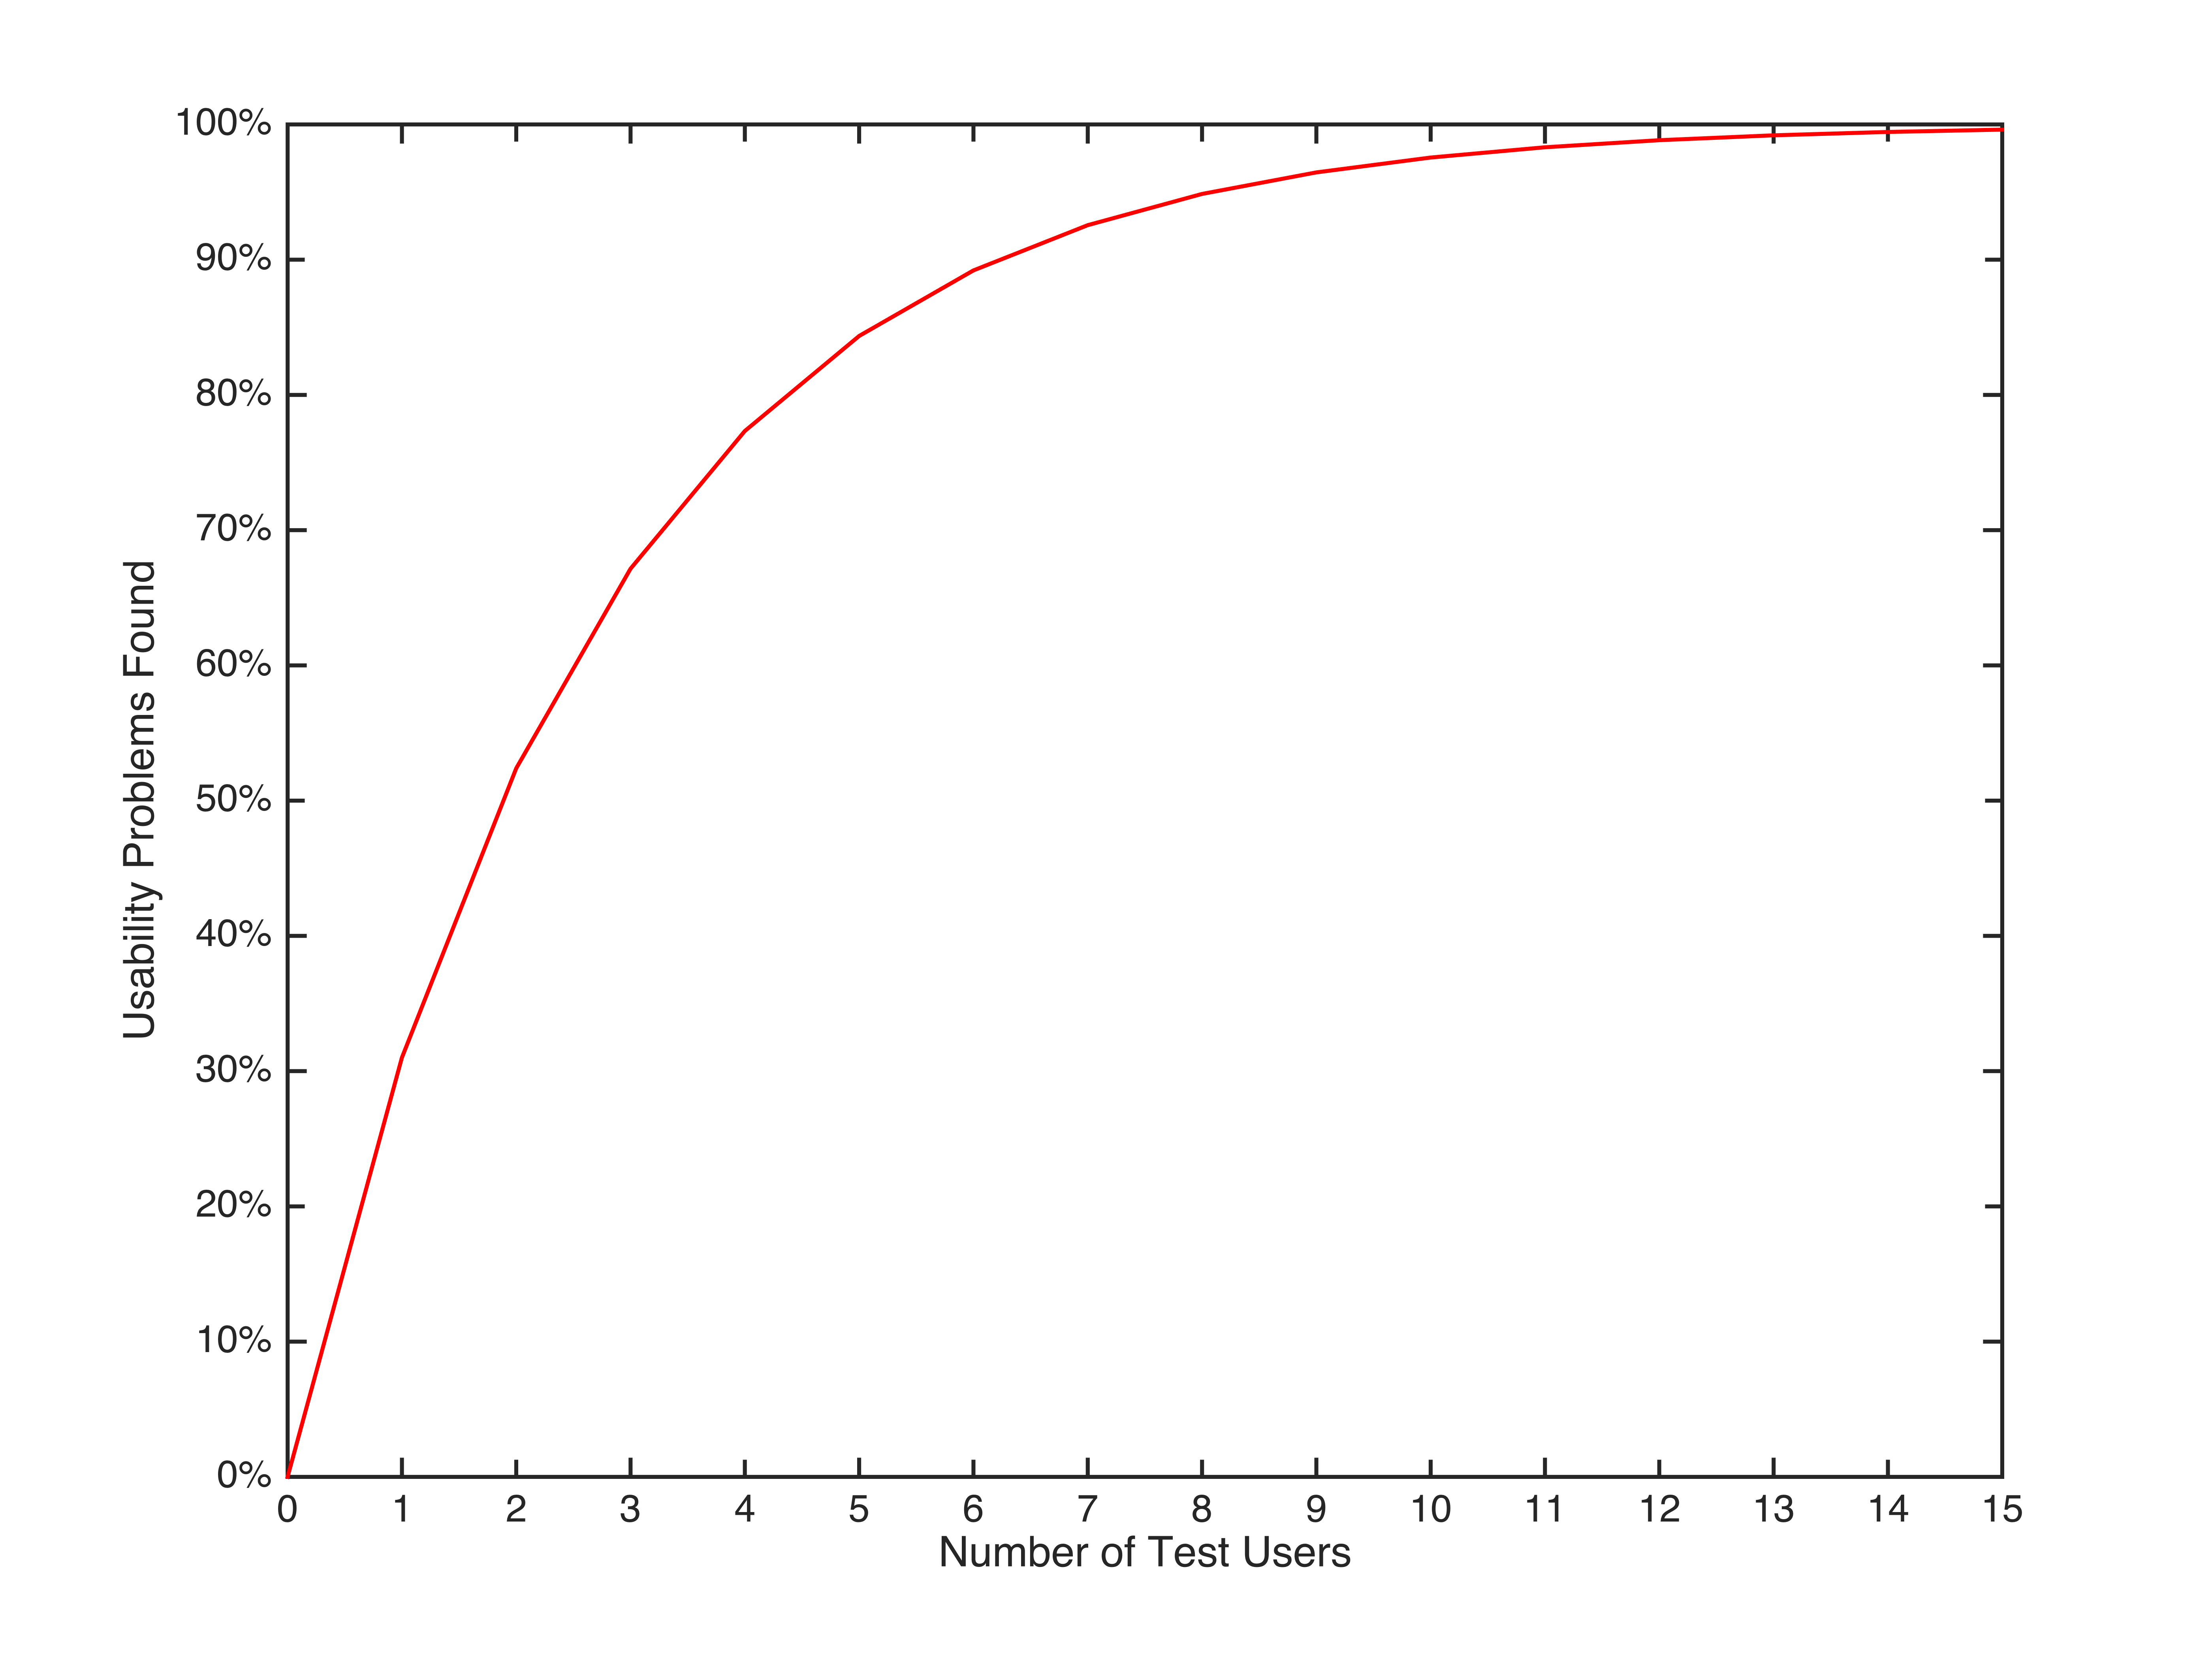
\includegraphics[width=0.8\textwidth]{Figures/eval-nielsen.png}
  \caption{Proportion of usability problems in an interface found by heuristic evaluation using various numbers of evaluators}
  \label{fig:eval-nielsen}
\end{figure}

\begin{itemize}
  \item  Interview type: Discussion and questions to be answered using a 5-point Likert scale with additional space for comments and feedback.
  \item  Number of questions: 10
  \item  Duration of each interview: 20-30 minutes
  \item  Time period of the conduction: 27th June 2016. The question sheet is attached to this thesis in Appendix \ref{appendix:interview}.
  \item  Interview conduction: 
  \begin{enumerate}
    \item Several courses are created at the very beginning before the interview is performed. 
    \item After the interview is started, interviewees are requested to sign up with their own accounts and search the certain course by the course code.
    \item Afterwards, they start questioning or answering within the certain course at the same time.
    \item Interviewees are also demanded to use the major functionalities of the system, especially the drawing tool and quote functionality.
    \item At last, the remaining 8 questions have been answered by the interviewees, followed by a final discussion of the results.
  \end{enumerate}
\end{itemize}

The overall results of the interviews are presented in table \ref{table:score-interview}, which contains the score rated by each interviewee and the average score of each question. 

\begin{table}[!htbp]
\centering
\begin{tabularx}{\textwidth}{@{}lXXXXXl@{}}
\toprule
Item(No.)       & A  & B  & C  & D  & E          & Average Score        \\ \midrule
1               & 5  & 4  & 4  & 5  & 5          & 4.6                     \\
2               & 4  & 5  & 5  & 4  & 4          & 4.4                     \\
3               & 5  & 4  & 4  & 5  & 4          & 4.4                     \\
4               & 4  & 3  & 4  & 3  & 4          & 3.6                    \\
5               & 4  & 3  & 3  & 3  & 2          & 3                     \\
6               & 4  & 5  & 4  & 5  & 4          & 4.4                     \\
7               & 5  & 5  & 5  & 5  & 4          & 4.8                     \\
8               & 2  & 3  & 3  & 2  & 2          & 2.4                     \\
9               & 3  & 4  & 5  & 4  & 3          & 3.8                     \\
10               & 2  & 3  & 1  & 2  & 1          & 1.8                     \\ \bottomrule    
\end{tabularx}
\caption{Score of each question in the interview}
\label{table:score-interview}
\end{table}

\subsubsection{Analysis of General Functionalities}
Question 1-3 are designed for evaluating the main workflow of the system. Relative high scores are made by interviewees while testing the main functionalities of the system such like searching for a certain course, submitting questions and answers.

One tester has raised the issue that the auto-generated code (e.g. \textit{dogP\_Iz8}) for querying the certain course is a little bit complex. Instead of a complex string with both alphabets and symbols, a simplified code which only has numbers would be accepted. In addition, interviewee C noticed that a pagination of the questions' list is required if the amount of question is getting greater.

\subsubsection{Analysis of Drawing Tool }
Question 4 is proposed to investigate the usability of the integrated text input in the drawing tool. Most interviewees are generally satisfied with the basic functionality of inputting a text string using the drawing tool. Tester B figured that the more stylings on the text should be implemented.

Most interviewees thought that the preset of the default elements were far not enough, which could be concluded from the Question 5. More shapes, which could be selected and drawn instantly, are highly required to be added into the preset. Otherwise, with the current elements of drawing shapes with the drawing tool, the expected graphical content is not able to be expressed precisely.

The history functionality of the drawing tool is productive according to the score rated in question 6. Undo/Redo function really helps the interviewees to correct the mistakes they made while using the drawing tool. Question 7 with the highest score shows that the modification on top of quoted content is convenient and useful.

\subsubsection{Analysis of Real-Time Functionality}

The real-time functionality is also investigated during the interview. All interviewees pointed out that the auto-ordering of answers is not seamless and inconspicuous, which could also cause distraction while viewing the answers. Therefore, the scores of question 8 and 10 are quite low.

However, the majority of interviewees has the opinion that the real-time feature will significantly improve the interactivity of the system despite of the distraction caused while auto-ordering is performed.

